\chapter{Environment Setup}
\label{ch:env}
In this chapter we describe the environment, libraries and tools we use to execute our tests.

In the following sections we install the SDKs to develop and interact with quantum computers from IBM and D-Wave. We also present two other useful tools to easily write optimization problems.

\section{Python environment}
The language used to interface with quantum computers is usually Python. In this section we create a virtual environment in Python in order to communicate with the IBM quantum computer and the D-Wave quantum computer.

For our tests we manage Python environments with \mintinline{sh}|conda|. Let's start by creating the virtual environment named \mintinline{sh}|quantum| and activating it with:
\begin{minted}{sh}
conda create --name quantum python=3.12 pip
conda activate quantum
\end{minted}
For our tests and to follow the various examples presented both by IBM and D-Wave, it is also useful to be able to run a Jupyter notebook. We can install Jupyter with:
\begin{minted}{sh}
pip install jupyter
\end{minted}

\section{IBM Qiskit}
To program a gate-based architecture and to access IBM quantum computers we use the \emph{Qiskit} software stack. The name Qiskit is a general term referring to a collection of softwares for executing programs on quantum computers.
\begin{figure}[H]
	\centering
	\includegraphics[width=.95\linewidth]{setup/overview-image}
	\caption{Qiskit software stack}
	\label{fig:qiskit_overview}
\end{figure}

The core components are \emph{Qiskit SDK} and \emph{Qiskit Runtime}. The first one is completely open source and allows the developer to define his circuit; the second one is a cloud-based service for executing quantum computations on IBM quantum computers.

\subsection{Hello World}
Following the IBM documentation\footnote{https://quantum.cloud.ibm.com/docs/en/guides/install-qiskit} we can install the SDK and the Runtime with:
\begin{minted}{text}
pip install qiskit matplotlib qiskit[visualization]
pip install qiskit-ibm-runtime
pip install qiskit-aer
\end{minted}

Line $3$ installs Aer, which is a high-performance simulator for quantum circuits written in Qiskit. Aer includes realistic noise models, and we will use it later to test our circuit.

Sometimes the Qiskit stack suffers from incompatibilities between the various software components that compose the environment. At the moment of writing, the latest packages seem to work without any problem. For our tests we will use \mintinline{py}|qiskit: 2.2.3|, \mintinline{py}|qiskit-ibm-runtime: 0.43.1| and \mintinline{py}|qiskit-aer: 0.17.2|.

If the setup is successful we are now able to run a small test to build a Bell state (two entangled qubits). The following code assembles the gates, shows the final circuit and uses a sampler to simulate on the CPU the result of $1024$ runs of the program.

\begin{listing}[H]
	\begin{minted}{py}
from qiskit import QuantumCircuit
from qiskit.primitives import StatevectorSampler

qc = QuantumCircuit(2)
qc.h(0)
qc.cx(0, 1)
qc.measure_all()

sampler = StatevectorSampler()
result = sampler.run([qc], shots=1024).result()
print(result[0].data.meas.get_counts())
qc.draw("mpl")
	\end{minted}
	\label{lst:hello_qiskit}
	\caption{Building Bell state}
\end{listing}

\subsection{Transpilation}
Each Quantum Processing Unit (QPU) has a specific topology. We need to rewrite our quantum circuit in order to match the topology of the selected device on which we want to run our program. This phase of rewriting, followed by an optimization, is called transpilation.

Considering, for now, a fake hardware (so we do not need an API key) we can transpile the quantum circuit \mintinline{py}|qc|, from the code above, to match the topology of a specific QPU:
\begin{listing}[H]
	\begin{minted}{py}
from qiskit_ibm_runtime.fake_provider import FakeWashingtonV2
from qiskit.transpiler import generate_preset_pass_manager

backend = FakeWashingtonV2()
pass_manager = generate_preset_pass_manager(backend=backend)

transpiled = pass_manager.run(qc)
transpiled.draw("mpl")
	\end{minted}
	\label{lst:transpilation}
	\caption{Transpilation}
\end{listing}
The following picture shows (\ref{fig:qc_orig}) the quantum circuit that builds a Bell state, and (\ref{fig:qc_trans}) the transpiled version where the Hadamard gate is replaced to match the actual topology of the QPU.
\begin{figure}[h]
	\centering
	\subfloat[Original circuit]
	{\label{fig:qc_orig}
		\includegraphics[height=2.8cm]{setup/bell_1}} \quad
	\subfloat[Transpiled circuit]
	{\label{fig:qc_trans}%
		\includegraphics[height=2.8cm]{setup/bell_2}} \\
	\caption{Transpilation example}
	\label{fig:qc_transpilation}
\end{figure}

\subsection{Execution}
To test our transpiled circuit we use Aer, which allows us to simulate also the noise of real quantum hardware. We can execute our program with:
\begin{listing}[H]
	\begin{minted}{py}
from qiskit_aer.primitives import SamplerV2

sampler = SamplerV2.from_backend(backend)
job = sampler.run([transpiled], shots=1024)
result = job.result()
print(f"counts for Bell circuit : {result[0].data.meas.get_counts()}")
	\end{minted}
	\caption{Simulated execution}
	\label{lst:execution}
\end{listing}

If we look at the results of the execution we can observe that some answers present non-entangled qubits; this is caused by the (simulated) noise of the quantum device. A typical output of the execution could be:
\begin{minted}{text}
> counts for Bell circuit : {'00': 504, '11': 503, '01': 10, '10': 7}
\end{minted}
Where states \mintinline{text}|01| and \mintinline{text}|10| should not be present in an ideal execution with no errors.

\subsection{A complete example on real hardware}

\section{D-Wave Ocean}
\label{sec:ocean}
To define an optimization problem that can be solved on a D-Wave quantum computer we use the Ocean software stack. Ocean also allows us to interact with D-Wave hardware, submit a problem, and simulate the execution on a classical CPU.
\begin{figure}[h]
	\centering
	\includegraphics[width=.95\linewidth]{setup/ocean_stack}
	\label{fig:ocean_overview}
	\caption{Ocean software stack}
\end{figure}

All tools that implement the steps needed to solve your problem on a CPU, a D-Wave quantum computer, or a quantum-classical hybrid solver can be installed with:
\begin{minted}{text}
pip install dwave-ocean-sdk
\end{minted}

After the installation, running the command \mintinline{sh}|dwave setup| will start an interactive prompt that guides us through a full setup. During the setup it is also possible to add an API token or connect to the D-Wave account to import a key directly to use the quantum hardware.

\subsection{Hello World}
To present a simple optimization program we consider the minimum vertex cover (MVC) problem. Given a graph $G = (V, E)$, the problem asks to find a subset $V' \subseteq V$ such that, for each edge $\set{u,v} \in E$, at least one of $u$ or $v$ belongs to $V'$, and the number of nodes in $V'$ ($|V'|$) is the lowest possible.

The reduction from MVC to an Ising formulation is well known. The cost function that we want to minimize can be expressed by:
\[
cost = \sum_{i = 1}^{|V|}v_i + 2 \cdot \sum_{\set{i,j} \in E}\left(1 - v_i - v_j + v_i v_j \right)
\]
where $v_i \in \set{-1, 1}$ and $v_i = 1$ means that $v_i \in V'$, otherwise $v_i = -1$.

Like all problems in Ising form we can express the cost as a symmetric matrix, so our function becomes
\[
cost = v^T \times \mathbf{M} \times v
\]
where $v$ is the vector containing the binary variables $v_i$.

The figure shows an example graph (\ref{fig:ising_ex_gr}) and the corresponding matrix (\ref{fig:ising_ex_mx}) expressing the cost function.

\begin{figure}[h]
	\centering
	\subfloat[Original graph]
	{\label{fig:ising_ex_gr}
		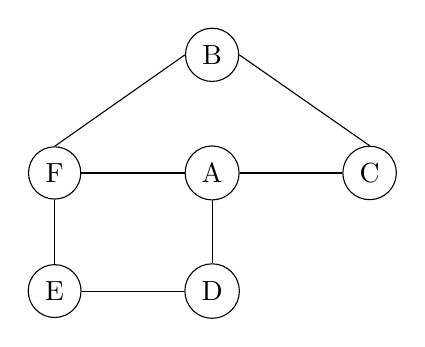
\begin{tikzpicture}
			\node (a) at (0,0)        [draw, circle] {A};
			\node (b) at (0,1.5)      [draw, circle] {B};
			\node (c) at (2,0)        [draw, circle] {C};
			\node (d) at (0,-1.5)     [draw, circle] {D};
			\node (e) at (-2,-1.5)    [draw, circle] {E};
			\node (f) at (-2,0)       [draw, circle] {F};
			\draw[-] (a.east)  -- (c.west);
			\draw[-] (a.south) -- (d.north);
			\draw[-] (a.west) -- (f.east);
			\draw[-] (b.east) -- (c.north);
			\draw[-] (b.west) -- (f.north);
			\draw[-] (d.west) -- (e.east);
			\draw[-] (e.north) -- (f.south);
		\end{tikzpicture}
	} \qquad
	\subfloat[Corresponding matrix]
	{
		\label{fig:ising_ex_mx}%
		\begin{tikzpicture}
			\node (a) at (0,0) {
				$
				\mathbf{M} = 
				\begin{pmatrix}
					1&0&2&2&0&2\\
					0&1&2&0&0&2\\
					0&0&1&0&0&0\\
					0&0&0&1&2&0\\
					0&0&0&0&1&0\\
					0&0&0&0&0&1\\
				\end{pmatrix}
				$
			};
		\end{tikzpicture}
	}
	\caption{Ising formulation}
	\label{fig:ising_ex}
\end{figure}

The following code presents a possible implementation of the Ising model described above. We have defined two dictionaries to store the matrix coefficients. The last line of code finds ten possible answers to the problem using the simulated annealing function implemented by D-Wave.
\begin{listing}[H]
	\begin{minted}{py}
from dwave.samplers import SimulatedAnnealingSampler
linear = {'A': 1, 'B': 1, 'C': 1, 'D': 1, 'E': 1, 'F': 1}
quadratic = {('B', 'C'): 2, ('B', 'F'): 2, ('C', 'A'): 2, ('D', 'A'): 2, ('E', 'D'): 2, ('E', 'F'): 2, ('F', 'A'): 2}
sampler = SimulatedAnnealingSampler()
result = sampler.sample_ising(linear, quadratic, num_reads=10)
	\end{minted}
	\caption{Ising example}
	\label{lst:ising_ex}
\end{listing}

If we print the results with \mintinline{py}|print(result.aggregate())| we can observe something similar to this:
\begin{minted}{text}
	A  B  C  D  E  F energy num_oc.
0 -1 -1 +1 +1 -1 +1  -14.0       6
1 +1 +1 -1 -1 +1 -1  -14.0       4
['SPIN', 2 rows, 10 samples, 6 variables]
\end{minted}
The two different results represent the two correct answers to our particular instance of the MVC problem.

\subsection{Example on real hardware}

\subsection{Minor embedding}

\section{PyQUBO and qubovert}
In listing \ref{lst:ising_ex} we have manually built the matrix representing the function that we want to minimize. It can be useful to have some tools that allow us to work at a higher level, defining cost functions like \ref{asd} that we defined in the section about quantum annealing (\ref{asd}).

Considering again the MVC problem, the objective function tends to minimize the number of nodes in our subset, while the penalty increases the cost if we leave out some edges. This interpretation allows us to transform the Ising model into the more familiar \textemdash{}from the point of view of a computer scientist\textemdash{} QUBO model, where all variables $x_i \in \set{0, 1}$. Let's see how PyQUBO and qubovert help us in this task.

\subsection{PyQUBO}
Reading from the documentation on the PyQUBO site\footnote{\url{https://pyqubo.readthedocs.io/en/latest/}}, PyQUBO allows us to create QUBOs or Ising models from flexible mathematical expressions easily. Some of the features of PyQUBO are:
\begin{itemize}
	\item Python based (C++ backend);
	\item Fully integrated with Ocean SDK;
	\item Automatic validation of constraints;
	\item Placeholder for parameter tuning.
\end{itemize}

We can install PyQUBO with \mintinline{text}|pip install pyqubo| and rewrite our MVC problem by defining the Hamiltonian that we want to minimize.
\begin{listing}[H]
	\begin{minted}{py}
from pyqubo import Binary, Placeholder, Constraint
from dwave.samplers import SimulatedAnnealingSampler

A, B, C, D, E, F  = Binary('A'), Binary('B'), Binary('C'), Binary('D'), Binary('E'), Binary('F')

H_objective = (A + B + C + D + E + F)
H_penalty = Constraint(((1 - A - C + A*C) +\
(1 - A - D + A*D) +\
(1 - A - F + A*F) +\
(1 - B - C + B*C) +\
(1 - B - F + B*F) +\
(1 - D - E + D*E) +\
(1 - E - F + E*F)) ,label='cnstr0')

L = Placeholder('L')
H = H_objective + L*H_penalty
H_internal = H.compile()
bqm = H_internal.to_bqm(feed_dict={'L': 2})

sampler = SimulatedAnnealingSampler()
result = sampler.sample(bqm, num_reads=10)
	\end{minted}
	\caption{Rewriting MVC with pyQUBO}
	\label{lst:MVC_pyQUBO}
\end{listing}

Listing \ref{lst:MVC_pyQUBO} presents a possible re-implementation of listing \ref{lst:ising_ex}, where we also see how PyQUBO interfaces with the Ocean SDK (line 17), and how to create (lines 14–16) and instantiate (line 17) a parametric Hamiltonian.

\subsection{qubovert}
As written in the documentation\footnote{\url{https://qubovert.readthedocs.io/en/latest/index.html}}, qubovert is the one-stop package for formulating, simulating, and solving problems in boolean and spin form. Using our nomenclature, boolean and spin form are respectively QUBO and Ising form.

Qubovert allows us to define various types of optimization problems that can be solved by brute force, with qubovert’s simulated annealing, or with D-Wave’s solver. Models defined in qubovert are:
\begin{description}
	\item [QUBO:] Quadratic Unconstrained Boolean Optimization;
	\item [QUSO:] Quadratic Unconstrained Spin Optimization (Ising model);
	\item [PUBO:] Polynomial Unconstrained Boolean Optimization;
	\item [PUSO:] Polynomial Unconstrained Spin Optimization;
	\item [PCBO:] Polynomial Constrained Boolean Optimization;
	\item [PCSO:] Polynomial Constrained Spin Optimization.
\end{description}

In addition to generic models, qubovert has a library of famous NP-complete problems mapped to QUBO and Ising forms.

\begin{listing}[H]
	\begin{minted}{py}
from qubovert import boolean_var
from dwave.samplers import SimulatedAnnealingSampler

A, B, C, D, E, F  = boolean_var('A'), boolean_var('B'), boolean_var('C'), boolean_var('D'), boolean_var('E'), boolean_var('F')

model = A + B + C + D + E + F
model.add_constraint_OR(A, C, lam=2)
model.add_constraint_OR(A, D, lam=2)
model.add_constraint_OR(A, F, lam=2)
model.add_constraint_OR(B, C, lam=2)
model.add_constraint_OR(B, F, lam=2)
model.add_constraint_OR(D, E, lam=2)
model.add_constraint_OR(E, F, lam=2)

qubo = model.to_qubo()
dwave_qubo = qubo.Q

sampler = SimulatedAnnealingSampler()
result = sampler.sample_qubo(dwave_qubo, num_reads=10)
	\end{minted}
	\caption{Rewriting MVC with qubovert}
	\label{lst:MVC_qubovert}
\end{listing}

Listing \ref{lst:MVC_qubovert} shows a possible implementation of the MVC problem using the tools provided by qubovert. Qubovert allows us to express our problem as a PCBO; we use this formulation to express constraints in a more natural way. In our example we ensure that each edge is covered simply by enforcing that at least one of the nodes linked by the edge is present in the solution. This constraint is repeated for each edge in the graph (lines 7–13). To specify the Lagrange multiplier (equation \ref{asd}) we use the keyword \mintinline{text}|lam|.

Qubovert, like PyQUBO, can interface with the Ocean SDK, transforming a PCBO problem into a QUBO problem (line 15) and then rewriting it in the format accepted by the D-Wave solver (or sampler).

\section{Conclusion}
In this chapter we have set up an environment to run our future experiments and tests. We have also shown some small examples to present the main characteristics and test the tools we will use in our work.

Following this setup allows anyone to recreate exactly the same configuration we use, avoiding (for what we know and test) incompatibilities between Python packages.
